\documentclass{article}

\usepackage[margin=2.54cm]{geometry}
\usepackage{setspace}

\usepackage[british]{babel}
\usepackage{csquotes}
\usepackage{hyperref}

\usepackage{titling}
\setlength{\droptitle}{-2cm}

\usepackage[backend=biber,style=alphabetic]{biblatex}
\addbibresource{\jobname.bib}

\usepackage{acronym}
\acrodef{ACT}{auto-correlation time}
\acrodef{ESS}{effective sample size}
\acrodef{HMC}{Hamiltonian Monte Carlo}
\acrodef{MCMC}{Markov chain Monte Carlo}
\acrodef{ODE}{ordinary differential equation}

\usepackage{mathtools}
\newcommand{\dd}{\, \mathrm{d}}
\renewcommand{\vec}[1]{\ensuremath{\boldsymbol{\mathbf{#1}}}}
\newcommand{\mat}[1]{\ensuremath{\boldsymbol{\mathbf{#1}}}}
\newcommand{\op}[1]{\ensuremath{\boldsymbol{\mathbf{#1}}}}
\newcommand{\norm}[1]{\ensuremath{\mathcal{N}\left(#1\right)}}

\usepackage{algorithm}
\usepackage{algpseudocode}

\usepackage{graphicx}
\usepackage{caption}
\usepackage{subcaption}
\captionsetup[ruled]{labelsep=period}

\title{Implementing \acl{HMC} for Efficient Bayesian Evolutionary Analysis \\
           \Large\textsc{awc summer scholarship report}}
\author{Arman Bilge \\ \texttt{\href{mailto:armanbilge@gmail.com}{armanbilge@gmail.com}}}
\date{22 April 2015}

\frenchspacing
\begin{document}

    \maketitle

    \subsection*{Introduction}

    Bayesian evolutionary analysis is centered around sampling from the
        posterior probability distribution of a phylogenetic
        tree~$\mathcal{T}$ and model parameters~$\vec\theta$
        given the molecular sequence data~$\mathcal{D}$~\cite{Bou+14},
        which by Bayes' theorem is
        \begin{equation}
            p\left(\mathcal{T}, \vec\theta \mid \mathcal{D}\right)
                \propto p\left(\mathcal{D} \mid \mathcal{T},\vec\theta\right)
                p\left(\mathcal{T} \mid \vec\theta\right) p\left(\vec\theta\right).
        \end{equation}
    Although direct sampling from this distribution is impossible, sampling
        strategies utilising \ac{MCMC} techniques~\cite{Met+53} have been quite
        successful~\cite{Ron+12,Dru+12,Bou+14}.
    The ideal sampling algorithm maximises the number of pseudo-independent
        samples drawn, called the \ac{ESS}, by minimising the correlation
        between consecutive samples.
    \ac{MCMC} generally performs poorly by this measure.
    Because the proposal distribution is ignorant of the target distribution,
        \ac{MCMC} exhibits random-walk behaviour and requires several steps to
        reach an uncorrelated sample~\cite{Nea11}.
    \ac{HMC}, first described as hybrid Monte Carlo~\cite{Dua+87},
        has the important advantage that the proposal distribution is the
        target distribution, enabling large changes to be made with each step.
    Computing an \ac{HMC} proposal involves solving a system of differential
        equations which is substantially more time-consuming than an \ac{MCMC}
        update.
    However, \textcite{Nea11} showed that, in theory, \ac{HMC} will outperform
        \ac{MCMC} as the problem dimensionality increases.
    I applied \ac{HMC} to Bayesian evolutionary analysis

    \subsection*{Methods}

    Let $\pi\left(\vec{q}\right)$ be the target probability density.
    We can consider a particle in our state space with position given
        by~$\vec{q}$ and momentum by $\vec{p}$.
    Then the Hamiltonian for our system is
        \begin{equation}
            H\left(\vec{q},\vec{p}\right)
            = U\left(\vec{q}\right) + K\left(\vec{p}\right)
        \end{equation}
        with potential energy
        $U\left(\vec{q}\right) = -\log{\pi\left(\vec{q}\right)}$ and kinetic
        energy $K\left(\vec{p}\right) = \frac{1}{2} \vec{p}^T \mat{M} \vec{p}$,
        where $\mat{M}$ is a positive-definite matrix that we interpret as
        the particle's mass.
    The system's dynamics are described by Hamilton's equations,
        \begin{equation}
            \frac{\dd \vec{q}}{\dd t} = \frac{\partial H}{\partial \vec{p}},
            \frac{\dd \vec{p}}{\dd t} = -\frac{\partial H}{\partial \vec{q}},
        \end{equation}
        which are integrated to find the state at a particular time.
    Typically this integration is achieved numerically using the leapfrog
        method~\cite{Nea11}.
    I use $\op{L}\left\{\vec{q},\vec{p}\right\}$ to denote an operator that
        maps the state at time~$t$ to the state at time~$t + \epsilon L$, as
        approximated by $L$~leapfrog steps with stepsize~$\epsilon$.
    Additionally, the momentum flip operator gives
        $\op{F}\left\{\vec{q},\vec{p}\right\}
         = \left\{\vec{q},-\vec{p}\right\}$.
    With the $\op{L}$ and $\op{F}$ operators we can reach a discrete set of
        states along an energy contour (subject only to errors in numerical
        integration).
    To guarantee ergodicity of the Markov chain, the momentum is randomised
        after each iteration of the algorithm by
        \begin{equation}
            \op{R}\left\{\vec{q},\vec{p}\right\} =
            \left\{\vec{q}, \sqrt{1-\alpha}\vec{p} + \sqrt{\alpha}\vec{n}\right\},
            \vec{n} \sim \norm{\vec{0}, \mat{M}^{-1}},
        \end{equation}
        where $\norm{\vec{\mu},\mat{\Sigma}}$ is the multivariate
        normal distribution with mean~$\vec{\mu}$ and covariance~$\mat{\Sigma}$.
    When the parameter $\alpha < 1$ the momentum is only partially refreshed,
        further suppressing random walk behaviour.
    Using these operators, the \ac{HMC} algorithm is concisely described by
        making repeated calls to the \textsc{HamiltonUpdate} function given in
        Algorithm~1.
    \begin{algorithm}
        \caption{A single iteration of the \acl{HMC} algorithm that uses
                 Hamiltonian dynamics to make the proposal and the Metropolis
                 criterion~\cite{Met+53} to accept or reject it.}
        \begin{algorithmic}[1]
        \Function {HamiltonUpdate}{$\left\{\vec{q},\vec{p}\right\}$}
            \State $\left\{\vec{q}^\prime, \vec{p}^\prime\right\}
                \leftarrow \op{F}\op{L}\left\{\vec{q},\vec{p}\right\}$
            \State $a \leftarrow \min\left(1,
                \exp\left(
                    H\left(\vec{q}, \vec{p}\right) - H\left(\vec{q}^\prime,
                        \vec{p}^\prime\right)\right)\right)$
            \State $\left\{\vec{q},\vec{p}\right\} \leftarrow
                \begin{cases}
                    \left\{\vec{q}^\prime, \vec{p}^\prime\right\}
                        & \text{with probability } a \\
                    \left\{\vec{q},\vec{p}\right\}
                        & \text{with probability } 1 - a
                \end{cases}$
            \State $\left\{\vec{q},\vec{p}\right\} \leftarrow
                        \op{R}\op{F}\left\{\vec{q},\vec{p}\right\}$
            \State \Return $\left\{\vec{q},\vec{p}\right\}$
        \EndFunction
        \end{algorithmic}
    \end{algorithm}

    I implemented the described \ac{HMC} algorithm in a fork of
        BEAST~v1.8~\cite{Dru+12}.
    In particular, I represented the \textsc{HamiltonUpdate} function as a
        standard \ac{MCMC} operator whose Hastings ratio is the exponential of
        the difference between the current and proposed kinetic energy.
    To enable evaluation of the gradient of the potential energy, I added a
        method \texttt{differentiate()} to the core \texttt{Likelihood}
        interface and implemented it for the basic probability distributions,
        coalescent and birth--death tree priors, and the Felsenstein tree
        likelihood~\cite{Fel81}.
    The tree likelihood implementation is optimised and makes use of the
        high-performance library BEAGLE~\cite{Ayr+12}.
    The source code for my fork is freely available under version 3 of the GNU
        General Public
        Licence\footnote{\url{https://github.com/armanbilge/B3/tree/hamilton}}.

    To evaluate the performance of \ac{HMC} relative to \ac{MCMC}, I simulated
        ten 32-taxa, ten 64-taxa, and ten 128-taxa datasets under the constant
        size coalescent and HKY substitution model with a strict molecular
        clock ($n = 2048$, $\theta = 0.5$, $\mu = 0.15$, $\kappa = 8.0$,
        $\vec{\pi} = \left[0.35, 0.30, 0.20, 0.15\right]$).
    I fixed the tree topology and model parameters to the truth and performed
        inference on the node heights using both \ac{MCMC} and \ac{HMC}.
    The \ac{MCMC} analysis used a auto-optimising scale operator on the root
        height and a uniform operator on all other node heights.
    The stepsize~$\epsilon$ for \ac{HMC} was auto-optimised during the analysis
        and nine different combinations were tried for
        $\left(L, \alpha\right) \in \left\{2, 4, 8\right\} \times \left\{0.33, 0.66, 1.0\right\}$.
    For optimal performance, the mass matrix $\mat{M}$ was set to the inverse
        of the covariance matrix for each dataset~\cite{Nea11}.
    I measured the performance of each algorithm as the minimum \ac{ESS} of
        all of the dimensions divided by the runtime, which is a
        theoretically-justifiable indicator of overall
        performance~\cite{Tho10}.

    \subsection*{Results and Discussion}

    In general, \ac{HMC} was either more efficient

    Given that this application of \ac{HMC} depends on the gradient of several
        non-trivial probability density functions, it is possible that there
        are still bugs in my implementation.
    The \ac{HMC} algorithm is very robust in the sense that errors in numerical
        integration will not prevent it from converging to the target
        distribution.
    However, this property makes it very difficult to debug, as problems do not
        affect correctness but only efficiency.

    \begin{figure}
        \centering
        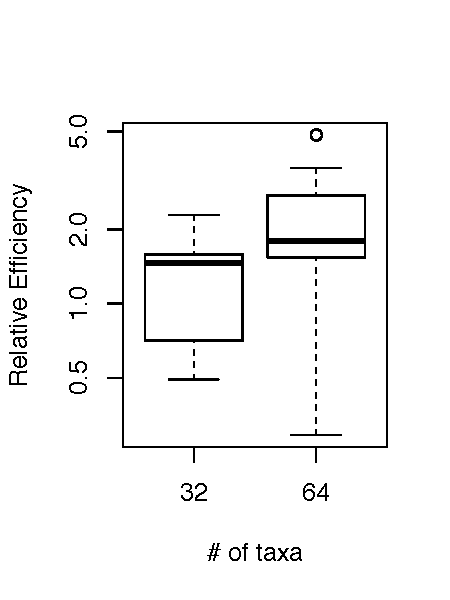
\includegraphics[scale=0.8]{boxplot.pdf}
        \caption{The efficiency of \ac{HMC} relative to \ac{MCMC} for the
                 thirty simulated datasets. The best-performing combination of
                 $L$ and $\alpha$ was taken as the representative \ac{HMC}
                 performance.}
    \end{figure}
    \begin{figure}
        \centering
        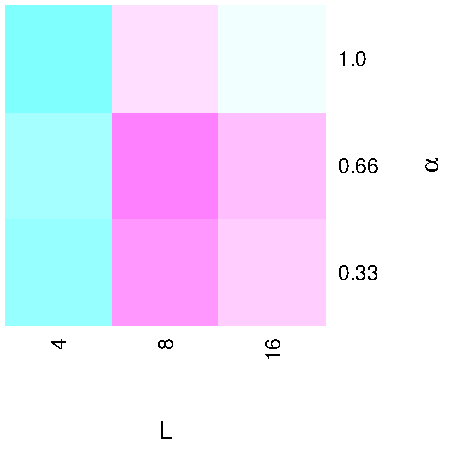
\includegraphics[scale=0.8]{heatmap.pdf}
        \caption{The efficiency of \ac{HMC} relative to \ac{MCMC} for various
                 values of $L$ and $\alpha$ for a particular 32-taxa dataset.
                 Magenta indicates that \ac{HMC} is more efficient and blue
                 otherwise.}
    \end{figure}

    \printbibliography

\end{document}
